\documentclass{ituhandin}

\coursename{Course name}
\fullname{Your name}
\when{January 2016}
\initials{init}
\coursecode{Course code}

\begin{document}
%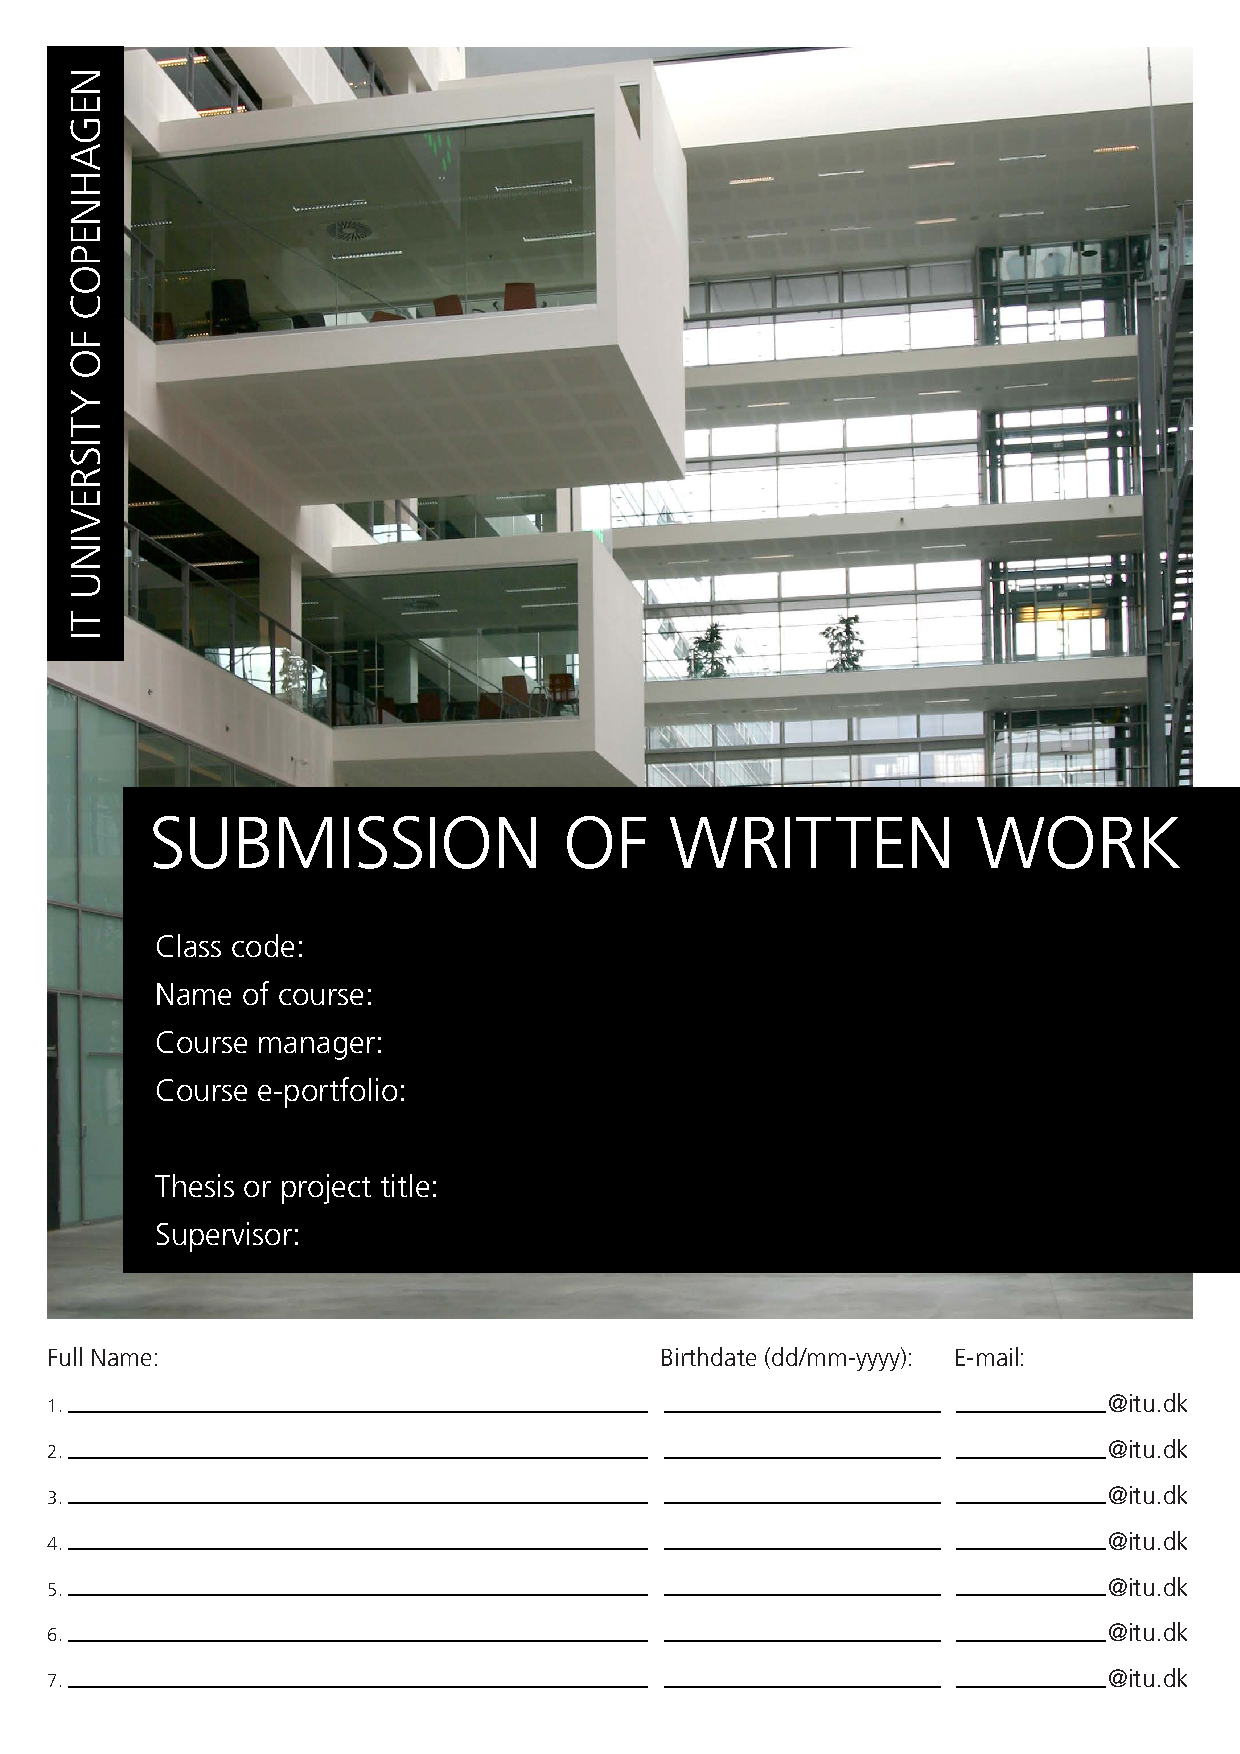
\includepdf{frontpage.pdf}
\maketitlepage
\signpage

\chapter{}

This is a fancy quote:
\fancyQuote{hej}{Niel Armstrong}

This is an even more fancier quote:
\moreFancyQuote{I am very fancy!}{Ludwig van Beethoven}

This is code in a box

\begin{lstlisting}[language=C, caption=This is a caption]
    void fac(int n, int *res) {
        if (n == 0)     /* fac's n */
        *res = 1;
        else {
            int tmp;
            fac(n-1, &tmp);
            *res = tmp * n;
        }
    }
\end{lstlisting}


This is code in the free

\begin{lstlisting}[language=ML, frame={}]
    let rec lookup env x =
    match env with 
    | []        -> failwith (x + " not found")
    | (y, v)::r -> if x=y then v else lookup r x;;

    type expr = 
    | CstI of int
    | Var of string
    | Prim of string * expr * expr;;
\end{lstlisting}


Happy exam! :-)


\chapter{}
\section{}
\section{}

\bibliographystyle{plainnat}
\bibliography{bibliography}

\styleAppendix
\appendix
\chapter{Some code}

\label{LastPage}
\end{document}
